\documentclass[runningheads]{llncs}
\usepackage{graphicx} 
\usepackage{xspace}
\usepackage{listings}
\usepackage{svg}
\usepackage[breaklinks=true,colorlinks,linkcolor=black,urlcolor=blue,citecolor=black]{hyperref}

\begin{document}
\title{A Graph Transformation-Based Engine for the Automated Exploration of Constraint Models}

\author{Christopher Stone \orcidID{0000-0002-9512-9987}
\and
András Z. Salamon \orcidID{0000-0002-1415-9712}
\and
Ian Miguel \orcidID{0000-0002-6930-2686}}
%
\authorrunning{C. Stone et al.}

\institute{School of Computer Science, University of St Andrews, UK
\email{\{cls29,Andras.Salamon,ijm\}@st-andrews.ac.uk}}

%\author{\fnm{Ian} \sur{Miguel}}\email{ijm@st-andrews.ac.uk} % {https://orcid.org/0000-0002-6930-2686}
%\author[1]{\fnm{András Z.} \sur{Salamon}}\email{Andras.Salamon@st-andrews.ac.uk}} % {https://orcid.org/0000-0002-1415-9712}


\newcommand{\essence}{\textsc{Essence}\xspace}
\newcommand{\conjure}{\textsc{Conjure}\xspace}
\newcommand{\savilerow}{\textsc{Savile Row}\xspace}
\newcommand{\code}[1]{{\texttt{#1}}}

\maketitle

\begin{abstract}
In this demonstration, we present an engine leveraging graph transformations for the automated reformulation of constraint specifications of combinatorial search problems. These arise in many settings, such as planning, scheduling, routing and design. The engine is situated in the Constraint Modelling Pipeline that, starting from an initial high-level specification, can apply type-specific refinements while targeting solvers from multiple paradigms: SAT, SMT, Mixed Integer Programming, and Constraint Programming. The problem specification is crucial in producing an effective input for the target solver, motivating our work to explore the space of reformulations of an initial specification.

Our system transforms a constraint specification in the \essence language into an Abstract Syntax Tree (AST). These ASTs, considered as directed labelled graphs, serve as inputs to the graph transformation language GP2 (Graph Programs 2) for subsequent reformulation. Our engine currently employs a curated set of handcrafted rewrite rules applied sequentially to the ASTs by the GP2 framework. It is designed to learn the efficacy of various rewrites, prioritising those that yield superior performance outcomes. At this stage, our primary emphasis is ensuring the rewritten specifications' soundness and semantic invariance.

Central to our methodology is constructing a search graph, where nodes represent model specifications and solutions, while edges represent graph transformations and solver performance. Through this search graph our system enables the exploration of constraint specification variants and the evaluation of their effects on lower-level refinement strategies and solvers.
Finally, we present a visualisation tool that allows the interactive inspection of the search graph and its content.
\end{abstract}

\keywords{Model Transformation
\and Constraint Programming
\and Graph Search}

\section{Introduction}

Combinatorial search problems arise in many and varied settings. Consider, for example, a parcel delivery problem. Parcels and drivers must be assigned to delivery vehicles respecting capacity constraints, staff resources, shift patterns and working preferences. At the same time routes must be chosen so as to meet delivery deadlines. The problem is further complicated by the need also to optimise an objective, such as minimising fuel consumption.

Such problems are naturally characterised as a set of decision variables, each representing a choice that must be made to solve the problem at hand (such as which items are assigned to the first van leaving the depot), and a set of constraints describing allowed combinations of variable assignments (for instance, a vehicle cannot be assigned to particular route depending on its specific height or weight). A solution assigns a value to each variable satisfying all constraints. Many decision-making and optimisation formalisms take this general form, including: Constraint Programming (CP), Propositional Satisfiability (SAT), SAT Modulo Theories (SMT), and Mixed Integer Programming (MIP). Metaheuristic methods offer a complementary approach, sacrificing completeness for the ability to explore rapidly a neighbourhood of candidate solutions. These approaches have much in common, but differ in the types of decision variables and constraints they support, and the inference mechanisms used to find solutions.

In all of these formalisms the {\em model} of the problem is crucial to the efficiency with which it can be solved. A model in this sense is the set of decision variables and constraints chosen to represent a given problem. There are typically many possible models and formulating an effective model is notoriously difficult. Therefore automating modelling is a key challenge. 

This work extends our {\em Constraint Modelling Pipeline}. A user writes a problem specification in the abstract constraint specification language {\sc Essence} \cite{frisch2008:essence}, capturing the structure of the problem in terms of familiar discrete mathematical objects such as sets, relations, functions, and partitions, but {\em without} committing to detailed modelling decisions. The {\sc Conjure} \cite{akgun2022conjure} automated modelling system refines an {\sc Essence} specification into a solver-independent constraint model where the abstract structure is represented by a collection of primitive variables and constraints. The second stage in the pipeline, performed automatically by {\sc Savile Row} \cite{savilerow}, is in preparing the model for a particular constraint solver for one of the formalisms listed above. By following different refinement pathways the pipeline can produce a set of alternative models from a single {\sc Essence} specification for evaluation or selection via machine learning. We have situated our work in the \essence language and constraint modelling pipeline because \essence allows problems to be expressed in a concise, highly structured manner. We exploit this structure to trigger the transformations we consider. 

The constraint modelling pipeline eliminates the need for specific modelling expertise in constraint programming and SAT solving.
However, the pipeline is sensitive to the way a problem is specified in \essence. This is because \conjure's refinement rules are triggered directly from the abstract variables and expressions in the {\sc Essence} specification, therefore determining the reachable set of models.
This motivates our work herein: an automated reformulation system to explore the space of {\sc Essence} specifications and therefore increase the size of the set of models from which we can select. Our tool uses graph formalisms throughout. An \essence specification is represented as a graph; all reformulations of an \essence specification are graph transformations. Specific properties can be preserved by transformations (such as semantic invariance), and rewrites are applied only when well-defined conditions are present. Furthermore our system uses a persistent data structure holding the history of previous reformulations, so supporting the accumulation of data for subsequent learning.

\section{Related Work}

To solve a constraint model of a problem efficiently, it is crucial to first choose an effective formulation for the model \cite{freuder2018:progress}.
Various approaches have therefore been proposed to automate the modelling process.
Methods learn models from, variously,
natural language~\cite{Kiziltan2016:constraint},
positive or negative examples~\cite{DeRaedt2018:learning,Bessiere2017:constraint,Arcangioli2016:multiple},
queries (membership, equivalence, partial, or generalisation)~\cite{Beldiceanu2012:model,Bessiere2013:constraint,Bessiere2014:boosting}, or
from arguments~\cite{Shchekotykhin2009:argumentation}.
% ALL \cite{coletta2003semi, lallouet_learning_2010, tsouros2018efficient};
Other approaches include:
automated transformation of medium-level solver-independent constraint models \cite{Rendl2010:thesis,Nethercote2007:minizinc,OPLBook,Mills1999:eacl,Nightingale2014:automatically,savilerow,Nightingale2015:automatically};
automatic derivation of implied constraints from a constraint model \cite{frisch2003:cgrass,colton2001:constraint,charnley2006:automatic,Bessiere2007:learning,Leo2013:globalizing};
case-based reasoning \cite{Little2003:using}; and
refinement of abstract constraint specifications \cite{Frisch2005:rules} in languages such as ESRA \cite{Flener2003:esra}, \essence \cite{frisch2008:essence}, ${\mathcal F}$ \cite{Hnich2003:function} or Zinc \cite{marriott2008:design,ZincModref10,Rafeh2016:linzinc}.

Model transformation by means of graph transformations \cite{mens2005use} has been applied successfully in a large variety of domains within software engineering, from databases and software architectures to visual languages\cite{kahani2019survey,taentzer2005model}.
Their application on automated test generation for debugging \cite{troya2022model} and automated software refactoring using local search are particularly relevant \cite{qayum2009local},
making its underlying mechanism an ideal candidate for implementing a system that allows us to explore variants of a constraint model rigorously.

% **** Chris should check
Weber \cite{weber2022tool} also implements a persistent data structure for a graph rewriting system, a feature at the heart of our system necessary for accumulating data in the prospect of subsequent learning. Automatic search of design spaces via machine learning approaches is highly desirable and has been sought-after in several fields, such as chip design \cite{hu2020machine} and has been implemented in the context of graph substitution guided by a neural network in \cite{jia2019taso}.

%Similarly to previous work \cite{weber2022tool}, our system uses a fully persistent data structure holding the history of previous graphs before transformations. This allows for more search paths to be available during model exploration and the 


\section{System description}

We now describe our overall system and the main format converters.

\subsection{Overview}

\noindent\textbf{Reformulating \essence Specifications via Graph Transformation.} The toolkit's core objective is rewriting \essence constraint specifications via graph transformations. This is implemented via an \essence parser that constructs an Abstract Syntax Tree (AST) of the specification, which preserves syntactic information by storing it as attributes and is then translated into a GP2 graph. Once translated, any available GP2 rewriting rule can be applied. The question then arises as to how to explore the space of \essence specifications. Since transformations can be chained sequentially, this process can be seen as balancing exploration and exploitation. For example, should a reformulated specification be reformulated (exploited) further or should we explore a new branch of the possible reformulation pathways?
This process can be treated as a multi-armed bandit problem~\cite{bandits-book}, informed by evaluating the models produced from the reformulated specification on training instances of the specified problem. Evaluation results are stored persistently to support the accumulation of knowledge and effective reformulations. 

%In the case of single instance specifications, the problem is solved and then solved again after each transformation while recording each step's performance. For parameterised specifications, an extra instance generation step is added.

\noindent\textbf{Persistent Knowledge Graph}. The exploration produces a persistent knowledge graph where nodes represent \essence specifications and solutions, while edges represent graph transformations, and evaluation results. The graph is implemented using the Python package NetworkX~\cite{networkx} as an attributed nodes and edges list. In practice, starting from a single node representing the initial specification, the knowledge graph is iteratively expanded by successfully applying a GP2 rewrite. Each new specification is evaluated, for a set of parameters if necessary, by refining and solving it, then adding new nodes and edges to the knowledge graph. A simple graph union operation can join knowledge graphs created during separate runs. The knowledge graph can be formatted as JSON or visualised using a web browser thanks to a custom procedurally generated HTML visualisation. The graph is translated into Force-Graph \cite{force_graph}, based on D3.js \cite{2011-d3}, which allows the visual inspection of the knowledge graph, the models and solutions that have been generated. This has already proven useful for examining the behaviour of the system and diagnosing programming errors during development.

\noindent\textbf{Format Translation Suite}.
Preparatory to the above, we have developed a collection of format converters that form a graph of available translations, pictured in Fig.~\ref{fig:FormatConverts}, that allows the conversion of the AST into NetworkX, GP2, Force-Graph, JSON, and can convert back to \essence itself. Some translations are necessary as intermediate steps to reach the GP2 language, while the complete suite allows users to access many tools for visualising, storing and analysing graphs. As the path from the GP2 language to NetworkX and JSON does not check or enforce compliance with \essence grammar the suite brings several further benefits beyond our specific goals. For example, the suite can be used independently to visualise and analyse arbitrary graphs specified in the GP2 language. Likewise, labelled NetworkX graphs can be converted to GP2, giving access to an extensive collection of graphs and graph generating functions.

\noindent\textbf{Python API Hub}. We implement our system in Python to facilitate interfacing with heterogeneous software, particularly {\sc Conjure} and GP2, acting as a portable, easy-to-access and easy-to-use hub. This enables users to run our system from Jupyter Notebooks and Colab, two popular choices for developing and sharing prototypes. Our wrapper around GP2 provides several quality-of-life features for managing graph transformations. For example, it can detect if a graph transformation rule is already compiled, automated on-the-fly compilation, or using pre-compiled programs generated with GP2.


\subsection{Format Converters}

We now describe some of the main format converters in our system.

\begin{figure}
\centering
  \includesvg[width = 295pt]{ICGT2024map.svg}
  \caption{Format Converters Graph}
    \label{fig:FormatConverts}
\end{figure}

\textbf{\essence string $\rightarrow$ \essence AST:} parses an \essence specification and returns a tree, as well as performing syntax and grammar checking. The AST is a typed rooted labelled directed tree where each node object stores its adjacency list. More formally it is a tuple $T : (N, A, n, t, l, A_n)$
\begin{itemize}
    \item $N$ and $A$ are a set of \textit{nodes} and ordered lists of \textit{nodes}.
    \item $t : N \rightarrow OBJECT$ maps each node to a set of types associated with \essence's grammar.
    \item $n : N \rightarrow A$ maps each node to an indexable ordered list of \textit{nodes}.
    \item $l : N \rightarrow STRING$ maps each node to a label holding an atomic unit of the \essence language.
    \item $A_n : N \rightarrow STRING$ maps each node to a set of attributes associated with \essence's grammar. This is redundant with $t$, but facilitates format conversion mechanics while $t$ facilitates the engineering of the parser.
\end{itemize}

\noindent\textbf{\essence AST $\rightarrow$ NetworkX(NX):} Converts a tree of python objects into a NetworkX graph by recursive traversal starting from the root.
When translating to NetworkX format it returns an attributed directed graph with vertex and edge labels. The node types are preserved as vertex attributes, and the children ordering is stored as edge attributes. More formally, the tree is turned into a tuple $G : (V, E, A_v,A_e, L_v)$ where
\begin{itemize}
    \item V is a set of vertices.
    \item $E \subseteq \{(u,v) | u,v \in V\}$ is a set of edges as ordered tuples with $u$ source and $v$ target.
    \item $A_v : V \rightarrow STRING$ are attributes associated with each vertex, storing grammatical information.
    \item $A_e : E \rightarrow INTEGER$ are attributes associated with each edge, holding the order of the target node.
    \item $L_v : V \rightarrow STRING$ are labels mapped to each vertex holding an atomic unit of the \essence language.
\end{itemize}

\noindent \textbf{NetworkX or \essence AST $\rightarrow$  GP2Graph:} When transforming a graph into GP2 graph format vertices are tuples of indices and labels while edges are quadruples of indices, source, target and labels. There are no \essence specific checks during this conversion and so it can be used for arbitrary graphs. Formally a GP2 graph is a tuple $G: (V_i,E_i,L_v,s,t,L_e)$
\begin{itemize}
    \item $V_i$ is a set of indexed vertices.
    \item $E_i$ is an indexed set of edges with $s$ source, $t$ target vertices from $V_i$.
    \item $L_v : V \rightarrow STRING$ are labels associated with each vertex, storing the grammatical information and atomic element.
    \item $L_e : E \rightarrow INTEGER$ are attributes associated with each edge, holding the order of the target node.
\end{itemize}


\noindent\textbf{NetworkX $\rightarrow$ \essence AST:} When converting from a NetworkX graph to an \essence tree, the tree's root must be found. We do this by topological sort, and start from the root to reconstruct the tree recursively.

\noindent\textbf{\essence AST $\rightarrow$ \essence String:} Compiling back to \essence is done by recursively traversing the tree and assembling the string according to the \essence syntax. We call this operation \textit{icing} as it mostly involves adding syntactic sugar.

\noindent\textbf{\essence AST $\leftrightarrow$ JSON:} We pack and unpack the nested Python objects using a standard JSON library.


In practice, the converters are not used in isolation but via an \essence Format Graph (EFG) module, with formats as vertices and converters as callable edges constructed by scanning and harvesting the functions in the Python module holding the converters via code introspection. Formally, it is a tuple $EFG : (V_f, E_c)$ where
\begin{itemize}
    \item $V_f$ is a set of vertices corresponding to each available format, which act as indices.
    \item $E_c : V \rightarrow CALLABLE$ is a pair $u,v \subseteq V_f$, a callable function that converts the input from the source format $u$ to the target format $v$.
\end{itemize}

The EFG module is used by specifying the source and target formats, then the shortest path is computed, and the input object is iteratively translated. For example, by using the method \code{EFG.FormToForm(input,"NX","GP2String")}, the path NX$\rightarrow$GP2Graph$\rightarrow$GP2String will be found. Then, the \emph{input} is passed to the source of the callable edge NetworkX $\rightarrow$ GP2Graph and then to the GP2Graph $\rightarrow$ GP2String, after these two conversions the outcome is returned.


\section{Transforming Models with Graph Transformations}

The driving engine of our system is an implementation of GP2 \cite{10.1007/978-3-319-40530-8_7}, a rule-based graph programming language which uses double pushout graph transformations. For a detailed explanation of the syntax and semantics of the language, see \cite{plump2017imperative}.
A Double Pushout Rule $p = (L, K, R)$ is a triplet of graphs known as the left-hand side $L$ that describes the precondition of the rule $p$, the right-hand side $R$ that describes its post-condition, and an interface $K$ that has to exist to apply the rule $p$. Applying the rule to a graph $G$ means finding a match $m$ of $L$ in the graph. This is used to create the context graph $D=(G-m(L))\cup m(K)$, in such a way that gluing of $L$ and $D$ via $K$ is equal to $G$, finally gluing $R$ and $D$ via $K$ leads to the final graph $H$.

In our system, the source graphs are always graph representations of valid ASTs of the \essence language, and we ensure that the rules we apply produce valid \essence ASTs after transformation. To control exactly which rules are applied, we keep each rule in separate files, trigger them one at a time, record if it is applied to the target graph and all the effects this has to the rest of the system. This includes the effects on \conjure and \savilerow, where the transformation could cause significant variations in the space or time required to refine the specification before passing it to the solver.


\subsection{Concrete Example}

We provide an illustrative simple example of an \essence specification and a graph transformation rule written in GP2 that can be applied to it. In the specification \ref{lst:before}, we have a Boolean parameter $a$, an integer parameter $b$ bounded between 1 and 10, a constant $c$ equal to 5 and a decision variable $d$, which is a Boolean that should satisfy the constraint described by the Boolean expression $a=!(d \land (b>c))$. The model's AST in its GP2 form, after all necessary format conversions have been applied, can be seen in the Appendix in Fig.~\ref{fig:demorg-BEFORE}. 

In Fig.~\ref{fig:demorgan}, we show the graphical form of a De Morgan rule implemented using GP2. Its raw string format can be found in Appendix \ref{lst:demorgGP2}. Applying the rule to the initial specification \ref{lst:before} leads to the new specification in \ref{lst:after}. The new specification is semantically equivalent, and the transformation has left intact the subtree of the expression $b>c$ as desired.

\noindent\begin{minipage}{.45\textwidth}
\begin{lstlisting}[caption=Original Specification,label={lst:before},frame=tlrb]{Name}
given a : bool
given b : int(1..10)
letting c be 5
find d : bool
    such that
        a = !(d /\ (b>c))
\end{lstlisting}
\end{minipage}\hfill
\begin{minipage}{.45\textwidth}
\begin{lstlisting}[caption=Rewritten Specification,label={lst:after},frame=tlrb]{Name}
given a : bool
given b : int(1..10)
letting c be 5
find d : bool
    such that
        a = (!d \/ !(b>c))
\end{lstlisting}
\end{minipage}


\begin{figure}[htbp]
\centering
  \includesvg[width=0.95\columnwidth]{demorgan.svg}
  \caption{De Morgan Rule implemented in GP2. Nodes n1,n3,n4 are the interface nodes.}
  \label{fig:demorgan}
\end{figure}

\section{Final Remarks and Future Directions}

With this demo we presented a new engine for exploring the space of reformulations of a constraint specification of a combinatorial search problem. The system allows the systematic testing of the Constraint Modelling Pipeline, the search for improved models of \essence specifications, the evaluation of reformulations that maintain the same level of abstraction, and gathering data useful for training model selection algorithms.

In the near term, we envision the system evolving towards the automated production of rewrite rules, starting from a pair of specifications. This allows the incorporation of good existing examples and expert modellers' knowledge without handcrafted rules but by rule derivation.
As we accumulate data, we will integrate machine learning algorithms and data driven approaches able to select models and drive the search for new improved models.

Our system is fundamentally designed around graphs. By introducing the ability to modify models and components via graph rewriting, we gained adaptability, reliability, and efficiency. As we extend our range of graph transformations, we expect to significantly advance the system's capabilities.

\newpage
\bibliographystyle{splncs04}
\bibliography{submission.bib}



\appendix

\section{Appendix}

\begin{lstlisting}[caption={A De Morgan rule implemented in GP2},label={lst:demorgGP2}]
Main = demorgFromNOTconjunction
demorgFromNOTconjunction(operand1,operand2:string)
//LHS
[
    (n1, "NOT~UnaryExpression")
    (n2, "AND~BinaryExpression")
    (n3, operand1)
    (n4, operand2)
    |
    (e1, n1, n2, 1)
    (e2, n2, n3, 1)
    (e3, n2, n4, 2)
]
=>
//RHS
[
    (n1, "OR~BinaryExpression")
    (n3, operand1)
    (n4, operand2)
    (n5, "NOT~UnaryExpression")
    (n6, "NOT~UnaryExpression")
    |
    (e4, n1, n5, 1)
    (e5, n1, n6, 2)
    (e6, n5, n3, 1)
    (e7, n6, n4, 1)
]
interface =
{
  n1,n3, n4
}

\end{lstlisting}

\begin{figure}[htb]
\begin{center}
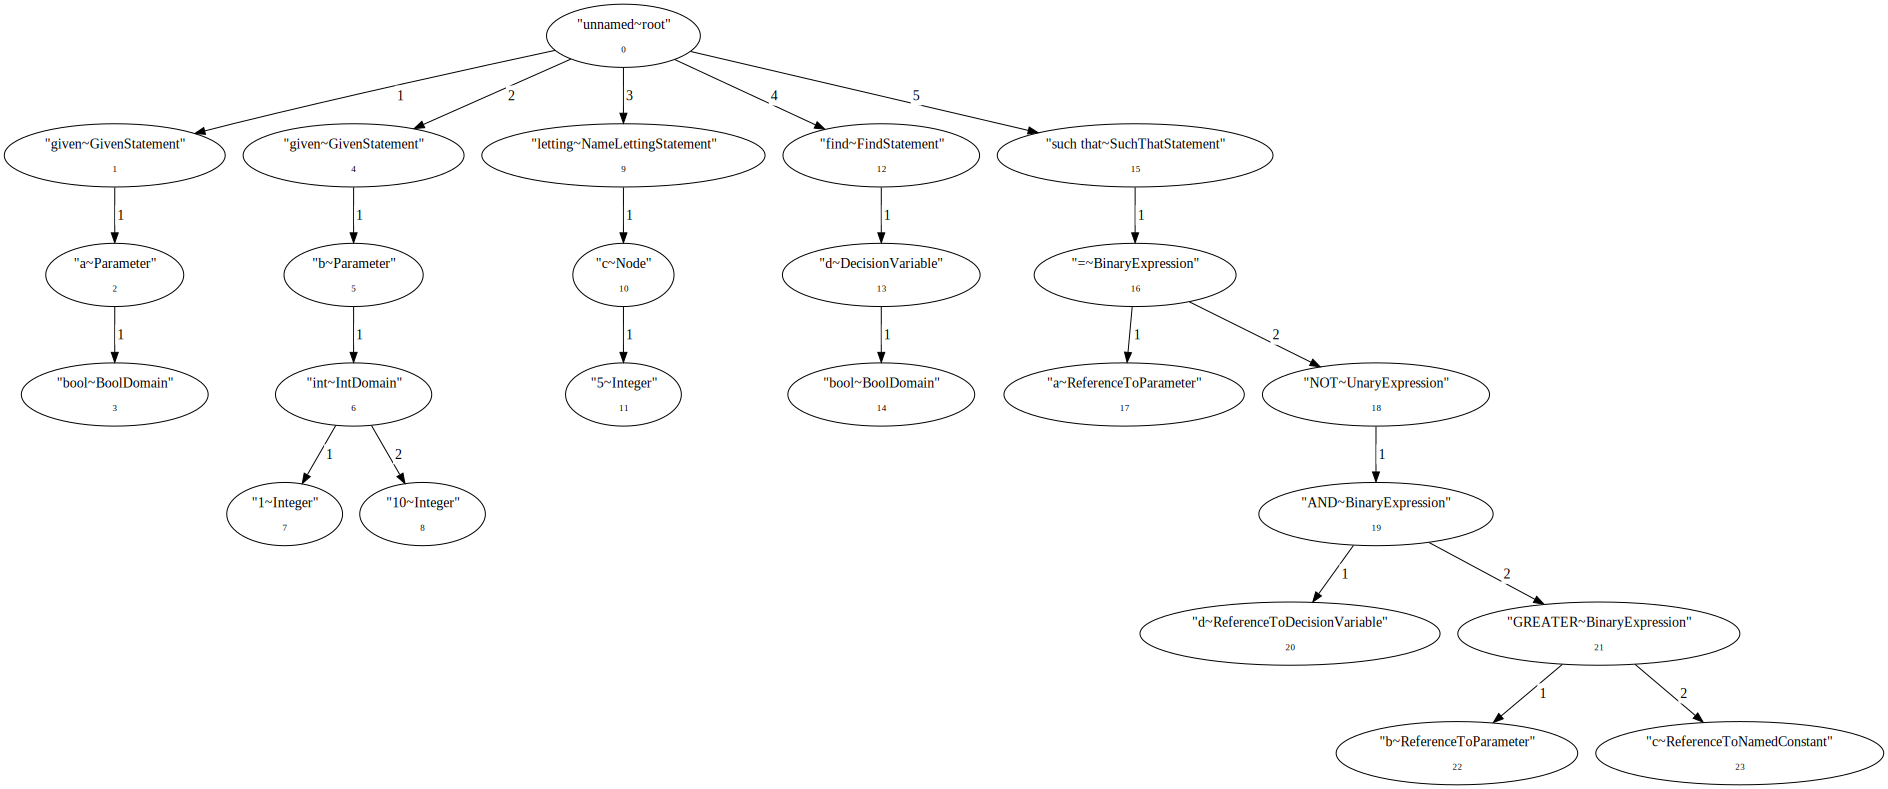
\includegraphics[angle=90,height=0.9\textheight,width=\textwidth]{demorg-BEFORE.pdf}
\caption{Example specification turned into GP2 before the application of the transformation}
\end{center}
\label{fig:demorg-BEFORE}
\end{figure}

\begin{figure}[htb]
\begin{center}
\includegraphics[angle=90,height=0.9\textheight,width=\textwidth]{demorg-AFTER.pdf}
\caption{Example specification turned into GP2 after the application of the transformation}
\end{center}
\label{fig:demorg-AFTER}
\end{figure}


\clearpage
\section{DEMO Appendix}


The demo's objective is to share our current progress and the tools we have already developed that could be useful to the broader graph transformation community.
Besides displaying our tools' features, we aim to interact with the graph transformation community for insights into applying more advanced and sound rewriting techniques and adjust our roadmap based on the feedback received. We will share a roadmap as part of the demo.
As principally constraint programming researchers, we are also interested in the role of constraint solving within the field of graph transformation for potential cross-pollination of ideas.

\subsection{Demo outline}

The demo will start by briefly introducing the Constraint Modelling Pipeline and its fundamental functions aided by Fig.\ref{fig:toolchain}. This will introduce the \essence language and its main features aided by a trivial introductory example.

Then the main overview of the system will look at the 3 graph protagonists of the paper aided by the diagram in Fig.~\ref{fig:GREEE}:
\begin{itemize}
    \item The Graph that represents an \essence specification.
    \item The Graph of format conversions that turns an \essence specification in various different forms.
    \item The Knowledge Graph that holds the history of the model exploration.
\end{itemize}

This will be followed by a live system run that construct and visualise a knowledge graph after each application of a graph transformation. Due to the interactive HTML nature of the visualisation, with features such as visualising the text of a specification by hovering over a node, this aspect of the system lends itself better to live presentation than PDF.

Then an advanced example will demonstrate a transformation applied to the Fractional Graph Colouring Problem specification, a generalisation of the graph colouring problem where more than one colour is associated with each vertex of a graph and the same colour can not be assigned to vertices connected by an edge. This will show how the system's main objective is realised and clarify the potential avenues of its use while highlighting the complexity within advanced rewrites.

The initial specification of the problem was used as a testbed for the system when it parsed only a smaller collection of types and graph problems naturally fit within relation types.

\begin{lstlisting}
given n : int(1..100)
letting vertices be domain int(0..n-1)
given edges : relation (irreflexive) of ( vertices * vertices )
given numberColours : int(1..n)
given coloursPerNode : int(1..n)
letting colours be domain int(1..numberColours)
find c : relation (size n*coloursPerNode) of ( vertices * colours )
such that
$ endpoints of edges do not share colours
    forAll (u,v) in edges .
        (forAll colourAssignment in c .
            (colourAssignment[1] = u) -> !((v,colourAssignment[2]) in c))

$ enforce number of colours per node, another version
    forAll u : vertices .
        coloursPerNode = (sum colourAssignment in c .
            toInt(colourAssignment[1] = u))
\end{lstlisting}


However, the solvers and pipeline could only handle instances of the problem as specified up to a specific size and complexity. 
After extending the parser and reformulating it as specified below, the refinement's time and space performance vastly improved, and so did solving time.
The main difference is that a constraint that lead to a counting task was substituted with an auxiliary variables that fixed the size of the number of colours needed. We will go through the steps required to perform this rewrite automatically.

\begin{lstlisting}
$ graph multicolouring for directed graphs
$ uses exactly coloursPerNode colours for each vertex
given n : int(0..100)
letting vertices be domain int(0..n-1)
given edges : relation (irreflexive) of (vertices*vertices)
given numberColours : int(1..n)
given coloursPerNode : int(1..n)
letting colours be domain int(1..numberColours)
letting coloursSet be domain set (size coloursPerNode) of colours
find c : function (total) vertices --> coloursSet
such that
    $endpoints of edges do not share colours
    forAll (u,v) in edges .
        c(v) intersect c(u) = {}
\end{lstlisting}

We will close by allowing an open conversation that we hope will be extended beyond the demo.

\begin{figure}
  \centering
  \includegraphics[width=0.75\linewidth]{toolchain.pdf}
  \caption{Automated Constraint Modelling Pipeline}
  \label{fig:toolchain}
\end{figure}

\begin{figure}
  \centering
  \includegraphics[width=\linewidth]{GREEE.jpg}
  \caption{Diagram of the System}
  \label{fig:GREEE}
\end{figure}


\end{document}

\end{document}


TEMPORARY BIN 


% \essence specifications are nodes, and edges are graph transformations in a higher level graph that fully preserves the history of rewrites applied by our systems. Our tool employs a collection of cross-format translations, which are nodes in a conversion graph. This allows the search for shortest paths between formats when multiple paths are available. This approach allows the extension of the available formats to require a single converter to access all the other formats or choose time-aware paths.




\noindent\begin{minipage}{.45\textwidth}
\begin{lstlisting}[caption=Before,frame=tlrb]{Name}
given a : bool
find b : bool
find c : bool
    such that
        a = !(b /\ c)
\end{lstlisting}
\end{minipage}\hfill
\begin{minipage}{.45\textwidth}
\begin{lstlisting}[caption=After,frame=tlrb]{Name}
given a : bool
find b : bool
find c : bool
    such that
        a = (!b \/ !c)
\end{lstlisting}
\end{minipage}

a collection of software, languages and formalisms that enable a user to express a combinatorial search problem in \essence, an abstract constraint specification language, capturing its structural properties beyond the level where modelling decisions are typically made. The modelling pipeline automatically generates a model from these specifications. This eliminates the requirement for user expertise in constraint modelling while retaining the specified problem's structure intact. The system can explore alternative models and leverage properties like symmetry (add more). This is implemented by applying a type-specific refinement via conjure, which translates the specification into \essence Prime which is further refined and translated into solver-specific languages across formalisms: SMT,MIP,SMT,SAT and CP (Improve this).

Until now, refinements have been applied while lowering the model's abstraction level. With this new tool, we enable transformations that are applied to and maintain the highest level of abstraction. 

The advantages are multifold:

\begin{itemize}
    \item Rewritten models are more humanly readable.
    \item It allows the study of high level choices on the entire pipeline plus solvers in a systematic manner.
    \item It enables the synthesis of abstract specification.
    \item We can be confident of property preserving rewrites.
\end{itemize}

All our formal rewrites make use of the GP2 language and compiler. As part of its integration with our tool we developed a Python interface for it, significantly improving its usability. Among other implemented features, such as invoking GP2 programs and reading results, it is possible to apply GP2 programs to arbitrary NetworkX graphs, Python's most popular graphs library.


Rest of the paper:

\begin{itemize}
    \item Explanation of the pipeline
    \item Diagram of our system
    \item Example of a transformation being applied - step by step - (projection on the graph colouring spec, relation to function, De Morgan)
    \item Explanation of the constructed `knowledge graph' with specs, solutions and transformations that have been applied (mention persistent history of graphs)
    \item Plot or screenshot of a graph showing the exploration
\end{itemize}
